% !TEX encoding = UTF-8
% !TEX TS-program = pdflatex
% !TEX root = ../arsclassica.tex
% !TEX spellcheck = it-IT

%************************************************
\chapter{Esperimenti numerici}\label{cap:esperimenti}
%************************************************
\omissis{}
% introdurre argomenti del capitolo (dataset, e quindi tsis + sperimentazione)
% introdurre modalità di sperimentazione
% introdurre cross-validation
% spiegare metriche di valutazione utilizzate? si!

\section{\Ds{1}}\label{sec:dataset-1}
Lo scopo di questa sezione è presentare il \ds{1} e i risultati di classificazione e apprendimento strutturale ottenuti (si vedano rispettivamente i capitoli~\vref{cap:ctbnc,cap:structurallearning}) utilizzando tale insieme di \emph{\keyword{dati completi}} come input.

\subsection{Modello TSIS}\label{subsec:tsis-simple-model}
Al fine di introdurre il \ds{1} è necessario presentare la rete stradale \acs{TSIS} e il relativo modello di simulazione \acs{CORSIM} da cui esso è stato generato.

\begin{sidewaysfigure}
\centering
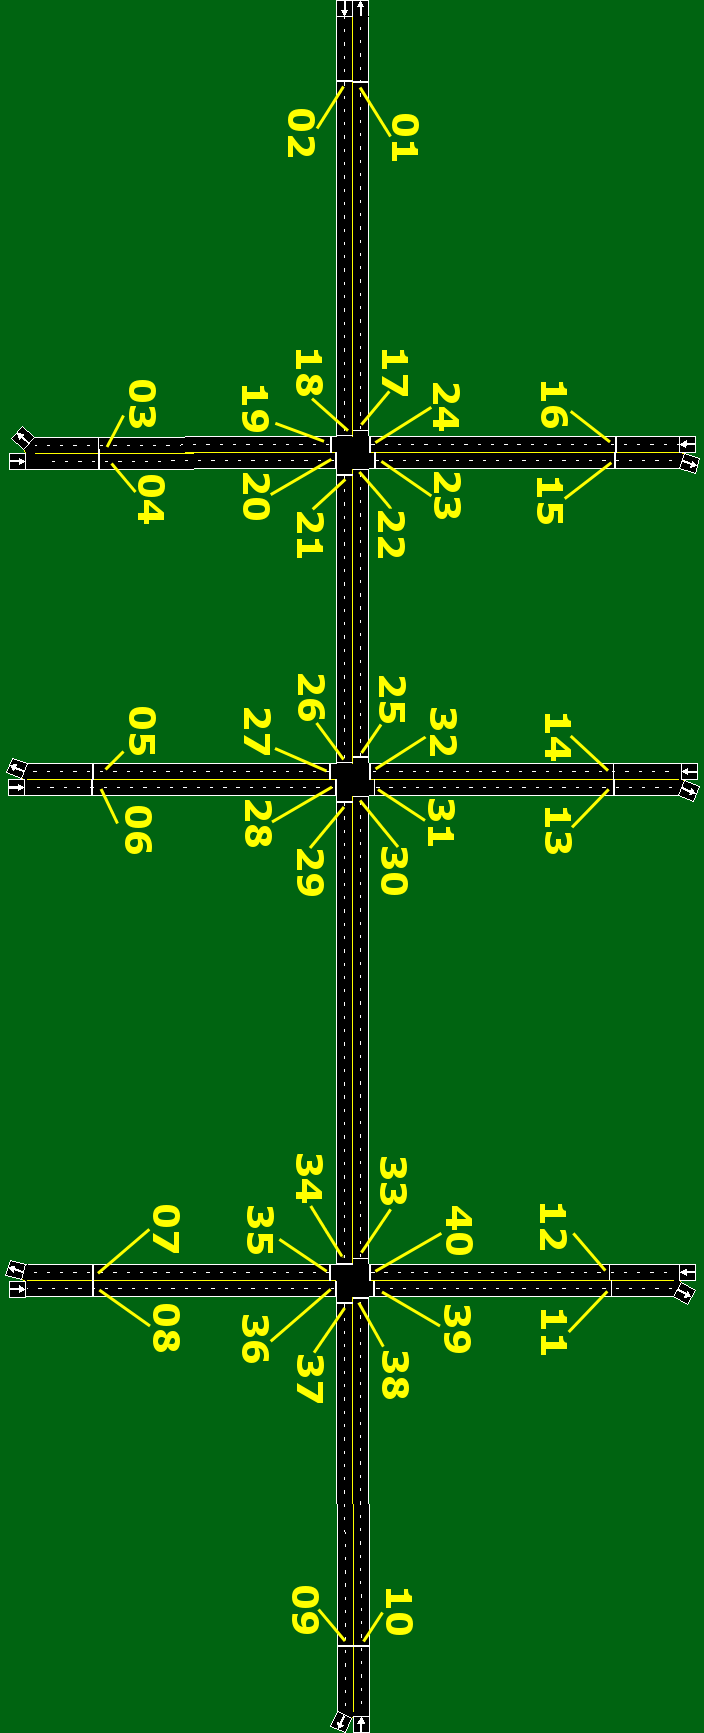
\includegraphics[width=1\columnwidth]{tsis-model-simple}
\caption[Rete stradale del \ds{1}]{File \acs{TNO} rappresentante la rete stradale da cui viene generato il \ds{1}.}
\label{fig:tsis-model-simple}
\end{sidewaysfigure}

\begin{table}[h]%
	\centering%
	\begin{tabular}{+l^l}
	\toprule\rowstyle{\bfseries}%
	\# & Sensore  \\\otoprule
	$01$& D$212$\\
	$02$& D$121$\\
	$03$& D$272$\\
	$04$& D$721$\\
	$05$& D$392$\\
	$06$& D$931$\\
	$07$& D$4412$\\
	$08$& D$1141$\\
	$09$& D$452$\\
	$10$& D$541$\\\bottomrule
	\end{tabular}
	\hspace{-0.6em}
	\begin{tabular}{+l^l}
	\toprule\rowstyle{\bfseries}%
	\# & Sensore  \\\otoprule
	$11$& D$4102$\\
	$12$& D$1041$\\
	$13$& D$382$\\
	$14$& D$831$\\
	$15$& D$262$\\
	$16$& D$621$\\
	$17$& D$211$\\
	$18$& D$122$\\
	$19$& D$271$\\
	$20$& D$722$\\\bottomrule
	\end{tabular}
	\hspace{-0.6em}
	\begin{tabular}{+l^l}
	\toprule\rowstyle{\bfseries}%
	\# & Sensore  \\\otoprule
	$21$& D$231$\\
	$22$& D$322$\\
	$23$& D$261$\\
	$24$& D$622$\\
	$25$& D$321$\\
	$26$& D$232$\\
	$27$& D$391$\\
	$28$& D$932$\\
	$29$& D$341$\\
	$30$& D$432$\\\bottomrule
	\end{tabular}
	\hspace{-0.6em}
	\begin{tabular}{+l^l}
	\toprule\rowstyle{\bfseries}%
	\# & Sensore  \\\otoprule
	$31$& D$381$\\
	$32$& D$832$\\
	$33$& D$431$\\
	$34$& D$342$\\
	$35$& D$4111$\\
	$36$& D$1142$\\
	$37$& D$451$\\
	$38$& D$542$\\
	$39$& D$4101$\\
	$40$& D$1042$\\\bottomrule
	\end{tabular}
	\caption[Sensori del \ds{1}]{Corrispondenza fra gli identificatori dei sensori del \ds{1} e l'indice con cui essi sono indicati nella~\autoref{fig:tsis-model-simple}.}
	\label{tab:ds-1-sensors-indices}
\end{table}

%immagine piano semaforico? no
%dire che ci sono (e dove sono) i semafori (l'immagine non li contiene), al massimo incollarli sull'immagine ...
%spiegare come è fatta la rete stradale e modello di simulazione del traffico: time period, semafori, come va il traffico durante i time period

\subsection{Risultati}
\omissis{}

%see: https://gist.github.com/leodido/5990626

\section{\Ds{2}}\label{sec:dataset-2}
\omissis{}

\subsection{Modello TSIS}\label{subsec:tsis-monza-model}
\omissis{}

% dire che parte da uno studio già fatto con sensori reali, riprodotto in tsis e esteso con altri sensori da me

\begin{table}[h]%
	\centering%
	\begin{tabular}{+l^l}
	\toprule\rowstyle{\bfseries}%
	\#  & Sensore \\\otoprule
	$01$& D$782$       \\
	$02$& D$781$       \\
	$03$& D$1687$      \\
	$04$& D$1681$      \\
	$05$& D$1682$      \\
	$06$& D$981$       \\
	$07$& D$982$       \\
	$08$& D$1480$      \\
	\end{tabular}
	\hspace{-0.6em}
	\begin{tabular}{+l^l}
	\toprule\rowstyle{\bfseries}%
	\#  & Sensore \\\otoprule
	$09$& D$892$       \\
	$10$& D$891$       \\
	$11$& D$192$       \\
	$12$& D$191$       \\
	$13$& D$1290$      \\
	$14$& D$912$       \\
	$15$& D$911$       \\
	$16$& D$1092$      \\
	\end{tabular}
	\hspace{-0.6em}
	\begin{tabular}{+l^l}
	\toprule\rowstyle{\bfseries}%
	\#  & Sensore \\\otoprule
	$17$& D$1091$      \\
	$18$& D$212$       \\
	$19$& D$211$       \\
	$20$& D$110$       \\
	\color{red}$21$& D$5098*$     \\
	\color{red}$22$& D$5099*$     \\
	\color{red}$23$& D$5097*$     \\
	$24$& D$421$       \\
	\end{tabular}
	\hspace{-0.6em}
	\begin{tabular}{+l^l}
	\toprule\rowstyle{\bfseries}%
	\#  & Sensore \\\otoprule
	\color{red}$25$& D$5096*$     \\
	$26$& D$321$       \\
	$27$& D$241$       \\
	$28$& D$242$       \\
	\color{red}$29$& D$5094*$     \\
	$30$& D$642$       \\
	\color{red}$31$& D$5095*$     \\
	$32$& D$541$       \\
	\end{tabular}
	\hspace{-0.6em}
	\caption[Sensori del \ds{2}]{Corrispondenza fra gli identificatori dei sensori del \ds{2} e l'indice con cui essi sono indicati nella \omissis{}}
	\label{tab:ds-2-sensors-indices}
\end{table}

Nella~\vref{tab:ds-2-sensors-indices}, i sensori il cui identificatore è contrassegnato da un asterisco corrispondono ai sensori reali, evidenziati anche nella figura \omissis{} tramite un indice numerico di colore rosso.

%varianti del dataset utilizzate
%split figure on more pages (search google is my friend)

\subsection{Risultati}
\omissis{}



%see: https://gist.github.com/leodido/5733991

%risultati:
%apprendimento
%classificazione (cross-validated)
%apprendimento strutturale (cross-validated)